Run this program for each method and produce a plot similar to Figure 4.2.

\begin{solution}\ \\\\
    We show the error per iteration for the boundary value problem $u''(x) = f(x)$ for the Jacobi, Gauss-Seidel, and
    Successive over-relaxation (SOR) methods below: \\\\

    \begin{figure}[h]
        \centering
        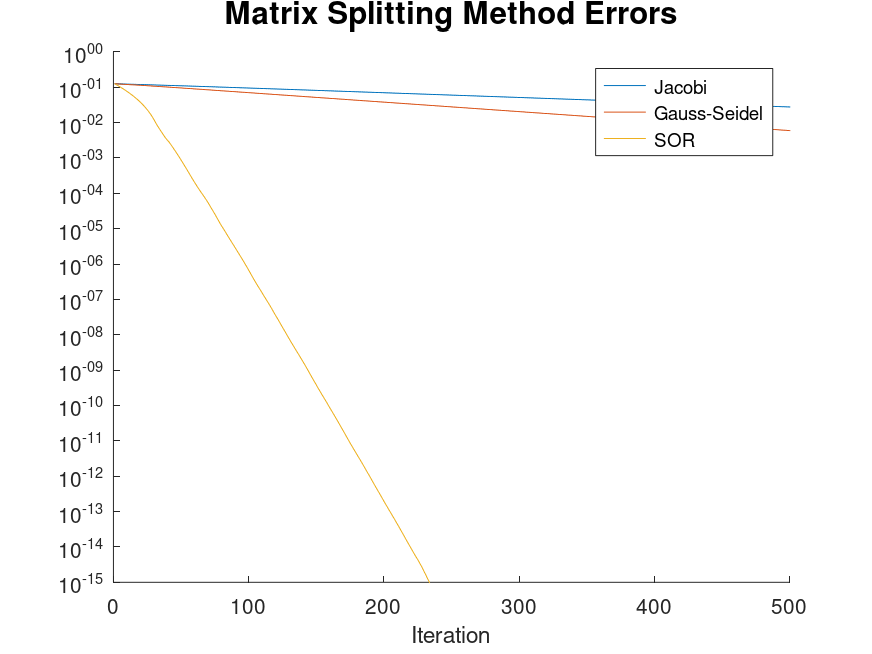
\includegraphics[width=.7\textwidth]{problem_1a_matrix_splitting_error_500_iterations.png}
        \caption[]{Comparison of matrix-splitting methods}
    \end{figure}

    As expected, we see that the SOR method converges radically faster than the Jacobi or Gauss-Seidel methods.
    \ \\\\
\end{solution}